\documentclass{llncs}
\usepackage{amssymb, amsmath}
\usepackage{makeidx}
\usepackage{graphicx}
\usepackage{tikz}
\usepackage{standalone}
\usepackage{url}

\usetikzlibrary{calc,trees,positioning,arrows,chains,shapes.geometric,%
  decorations.pathreplacing,decorations.pathmorphing,shapes,%
  decorations.text, fit, shapes.geometric, hobby, backgrounds, calc,
  matrix,shapes.symbols,plotmarks,decorations.markings,shadows}

\newcommand{\ignore}[1]{}
\newcommand\todo[1]{\textcolor{blue}{[TODO: #1]}}

%
\begin{document}
%
\mainmatter
%
\title{Automatic Generation of Transit Maps}
%
\titlerunning{Automatic Generation of Transit Maps}
%
\author{Hannah Bast\inst{1} \and Patrick Brosi\inst{1} \and
Sabine Storandt\inst{2}}
%
\authorrunning{Hannah Bast et al.} % abbreviated author list (for running head)
%
%%%% list of authors for the TOC (use if author list has to be modified)
\tocauthor{Hannah Bast, Patrick Brosi, Sabine Storandt}
%
\institute{University of Freiburg (Germany)\\
\email{\{bast, brosi\}@informatik.uni-freiburg.de}
\and
JMU W\"urzburg (Germany)\\
\email{storandt@informatik.uni-wuerzburg.de}
}

\maketitle

\begin{abstract}
	\todo{abstract}
\keywords{computational geometry, graph theory, optimization}
\end{abstract}


%
\section{Introduction}\label{SEC:intro}
%
\begin{itemize}
	\item mention usefulness, mention bad google maps etc
	\item mention that we know of no publication adressing the MCLM or the drawing of metro maps that uses real-world data
	\item mention that we not only want to generate schematic maps, but maps that resemble the real-world vehicle paths as closely as possible (e.g. to serve as a map overlay)
\end{itemize}
\todo{introduction, show some example map, either rendered by us or a manually created one to set the mood}

%
\subsection{Related Work}\label{SEC:related}
%

In \cite{ben06}, the problem of minimizing intra-edge crossings in transit maps was introduced with the premises of not hiding crossings under station markers for aesthetic reasons. A polynomial time algorithm for the special case of optimizing the layout along a single edge was described. The term metro-line crossing minimization problem (MLCM) was coined in \cite{bek07}. In this paper, optimal layouts for path and tree networks were investigated but arbitrary graphs were left as an open problem. In \cite{arg08}, \cite{nol09}, \cite{arg10}, several variants of MLCM were defined and efficient algorithms were presented for some of those, often with a restriction to planar graphs. In \cite{asq08}, an ILP formulation for MCLM under the periphery condition \todo{explain here?} was introduced. The resulting ILP was shown to have a size of $\mathcal{O}(|L|^2 \cdot |E|)$ with $L$ being the set of metro lines and $E$ the set of edges in the derived graph. In another line of research, it was observed that many (unavoidable) crossings scattered along a single edge are also not visually pleasing, hence the idea to group crossings into block crossing was exploited \cite{fin13b}. The problem of minimizing the number of block crossing was proven to be NP-hard on simple graphs just like the original MCLM problem \cite{fin13a}. As far as we are aware there are no papers on MLCM concerned with real data or containing an experimental evaluation.

The other crucial difference of all these approaches to our work is the strong abstraction from the geometry of the transit map. In all papers listed above, the graph used for optimization is constructed upon the stations which serve as nodes and the transit lines which induce edges between those nodes. But the original embedding of the edges is not taken into account, and crossings are allowed to occur anywhere along the edges (except their endpoints). As we aim for a truthful presentation of vehicle paths in our transit map, we do not ignore the shape of the lines between stations.  Instead, we introduce a new graph model for transit maps where nodes represent topology changes in the embedding and edges represent parallel line segments. This allows us to restrict crossing events to nodes (without hiding them behind station markers!). Our approach resolves some issues with the MLCM model, as e.g. the restricted applicability of some algorithms to planar graphs, and the necessity of artificial grouping of crossings (which happens naturally with our approach).

%
\subsection{Contribution}\label{SEC:contrib}
%
\begin{itemize}
	\item We introduce an approach for drawing transit maps that can be used with arbitrary input data in the GTFS format
	\item ... describe a simple line-sweeping approach to extract the spatial topology graph of a set of (partially overlapping) polylines
	\item ... describe a baseline ILP for solving the metro line crossing problem (MLCM)
	\item ... describe a improvied ILP for solving (MLCM) and add a simple extension that also minimizes line-separations (and subsequently, a special case of the periphery problem (MLCM-P))
	\item ... describe some heuristics for placing inevitable crossings in a asthecitally pleasing way
	\item ... describe the reduction of the minimization problem to core problem graphs which simplifies the problem
\end{itemize}

\todo{write contributions}

%
\subsection{Problem Definition}\label{SEC:def}
%
Let $L$ by a set of unique transit lines and w.l.o.g. $l \in \mathbb{N}$. We call an undirected graph $T = (V, S)$ with vertices $v = (p_v, \sigma_v)$ and segments $s = (u, v, L(s), \tau_s)$ a transit graph. Each $v$ has a position $p_v \in \mathbb{R}^2$. Furthermore we assign each segment $s$ a polygonal chain $\tau_s = (p_1, ..., p_n), p_i \in \mathbb{R}^2$ which describes the geometrical path a segment takes through the plane. For each $s$, we impose $p_1 = p_u$ and $p_n = p_v$, that is the polygonal chain has to start and end at the position of the segment's start and end node. $L(s)$ is the (ordered) set of lines that traverse $s$. Finally, we assign each node a role $\sigma_v \in {0, 1}$. If $\sigma_v = 1$, then we say that $v$ is a real station node. If $\sigma_v = 0$, we call $v$ a spatial topology node. A spatial topology node is a node where two or more lines diverge.

\todo{some real-world transit graph example (maybe Freiburg?)}
% \begin{figure}[h]
% \centering
%	\includestandalone[width=5cm]{tikz/transitgraph_small}
%	\caption{A transitgraph.}
%\end{figure}

$G$ can be understood as an embedding of an undirected multigraph $G = (V, E)$, where each line $l$ traversing a segment $s$ is transformed into a single edge. It can also be understood as an embedding of a set of $\mathbb{L}$ polygonal chains.
The goal is to render $T$ in a way that resembles a modern transit map.
We chose this definition because it proved to be useful during line-ordering optimization as well as during map rendering (see Section~\ref{SEC:rendering}). It also resembles the intuitive understanding of a transit map.

\todo{mention in further work (or somewhere more appropriate) that it is very easy (as we have done it) to apply our approach to a directed graph.}

%
\section{Spatial Topology Extraction}\label{SEC:topo}
%

Real-world public transit data is usually given as a set of vehicle trips. A trip is an ordered list of served stations. The vehicle's geographical path may also be given. In recent years, the General Transit Feed Specification (GTFS) has become the dominant format for exchanging public transit schedules.

Because each trip is given explicitely, the embedded transit graph $T$ induced by this data has many overlapping edges that may (partially) share the same geographical path.

Let $e_1, e_2$ be two edges in $T$ with their geometrical paths $\tau_{e_1}$ and $\tau_{e_2}$. We define a parametrization $\tau(\pi): [0,1] \mapsto \mathbb{R}^2$ which maps the progress $\pi$ to a point $p_d$ on $\tau$. For some distance threshold $\hat{d}$, we say $((\pi_1, \pi_2), ({\pi'}_1, {\pi'}_2))$ is a shared segment of $e_1$ and $e_2$ iff \[\forall (\pi, \pi'), \pi \in [d_1, {d'}_1], \pi' \in [d_2, {d'}_2] : \|\tau_{e_1}(\pi) - \tau_{e_2}(\pi')\| \leq d,\]

where $\|p - p'\|$ is the euclidean distance between $p$ and $p'$.

We transform $T$ into a well-formed transit graph $T'$ by repeatedly collapsing shared segments between two edges $e_1, e_2$ into a single new edge $e_{12}$ until no shared segments can be found. If for any of the edges the start of the shared segment $\pi$ lies not at the beginning of $\tau_e$, we split $e = (u, v)$ at $\pi$ into two edges $e'$ and $e''$ and introduce a new topological node $v'$ such that $e' = (u, v')$ and $e'' = (v', v)$ as well as $\tau_{e'}(1) = \tau_{e}(pi)$ and $\tau_{e''}(0) = \tau_{e}(pi)$. The same goes for the end point of a shared segment.

To find the shared segments between two paths $\tau$ and $\tau'$, we do a simple sweep over $\tau$ in $n$ steps of some $\Delta\pi$, measuring the distance $d$ between $\tau(i\cdot\Delta\pi)$ and $\tau'$ at each $i < n$ along the way. If $d \leq \hat{d}$, we start a new segment. If $d > \hat{d}$ and a segment is open, we close it. The algorithm can be mode more robust against outliers by allowing $d$ to exceed $\hat{d}$ for a number of $n$ steps.

\todo{example figure}
% \begin{figure}[h]
% \centering
% \includestandalone[width=\textwidth]{tikz/linecollapse}
% \caption{Line sweeping algorithm for spatial topology extraction}
% \end{figure}
The process can be sped up by indexing every linear segment of every vehicle path in a geometric index (for example, an R-Tree), making for a better lookup time of nearby segments.

%
\section{Line Ordering Optimization}\label{SEC:ordering}
%
We want to optimize the ordering imposed on each $s \in S$ in such a way that single lines can be easily traced through the network and the rendered map looks visually pleasing. These rather subjective criteria are usually formulated as the problem if minimizing the number of line crossing in the map (see Fig.~\ref{FIG:crossings}). This is commonly called the Metro Line Crossing Minimization Problem (MLCM). ? and ? suggest that it may improve the readability of the map if lines ending in a station only occur on the left or right side of the ordered sequence of a segment. This is called the periphery condition. MLCM under the periphery condition is called MLCM-P.

In this section, we describe a baseline integer linear program (ILP) to solve MLCM with $\mathcal{O}(|S|M^{2})$ variables and $\mathcal{O}(|S|M^{6})$ constraints.
We introduce an improved version of this program that only needs $\mathcal{O}(|S|M^2)$ constraints and describe an extension to this ILP which solves MLCM under the line separation constraint \todo{maybe call this MLCM-S?}
MLCM-S tries to avoid the separation of lines that traverse a segment $s$ next to each other in an adjacent segment $s'$ (see Section~\ref{SEC:separation}).
This has several benefits and also covers a special case of MLCM-P which we think is the most important.

%
\subsection{Baseline ILP}\label{SEC:baseline}
%
For every segment $s \in S$, we define $|L(s)|^{2}$ decision variables $x_{slp} \in \{0,1\}$ where $s$ indicates the segment, $l \in L(s)$ the line, and $p=1, \cdots, |L(s)|$ the position/number of the edge in the segment. We want to enforce $x_{slp}=1$ when line $l$ is assigned to edge number $p$ in the segment, and $0$ otherwise. This can be realized as follows:
\begin{equation*}
\forall l \in L(s): \sum_{p=1}^{L(s)} x_{slp}=1.
\end{equation*}
To assure that each edge get assigned exactly one line, we additionally need the constraints:
\begin{equation*}
	\forall p \in  \{1,\cdots,|L(s)|\} : \sum_{l \in L(s)} x_{slp} = 1.
\end{equation*}
% \smallskip\\
% \textbf{Example:}
% \begin{center}
% $x_{sA1} + x_{sA2} + x_{sA3} = 1$\\
% $x_{sB1} + x_{sB2} + x_{sB3} = 1$\\
% $x_{sC1} + x_{sC2} + x_{sC3} = 1$\smallskip\\
% $x_{sA1} + x_{sB1} + x_{sC1} = 1$\\
% $x_{sA2} + x_{sB2} + x_{sC2} = 1$\\
% $x_{sA3} + x_{sB3} + x_{sC3} = 1$\smallskip\\
% $x_{sA1}, x_{sA2}, x_{sA3}, x_{sB1}, x_{sB2}, x_{sB3}, x_{sC1}, x_{sC2}, x_{sC3} \in \{0, 1\}$
% \end{center}
\subsubsection{Avoiding crossings}\label{SEC:ac}
Let $A, B$ be two lines belonging to a segment $s$ over vertices $v,w$ and both extend over $w$. We distinguish two cases: Either there is an adjacent segment $s'$ with $A,B \in L(s')$ as well or $A$ and $B$ continue in different segments.
\begin{figure}
  \centering
	$\vcenter{\hbox{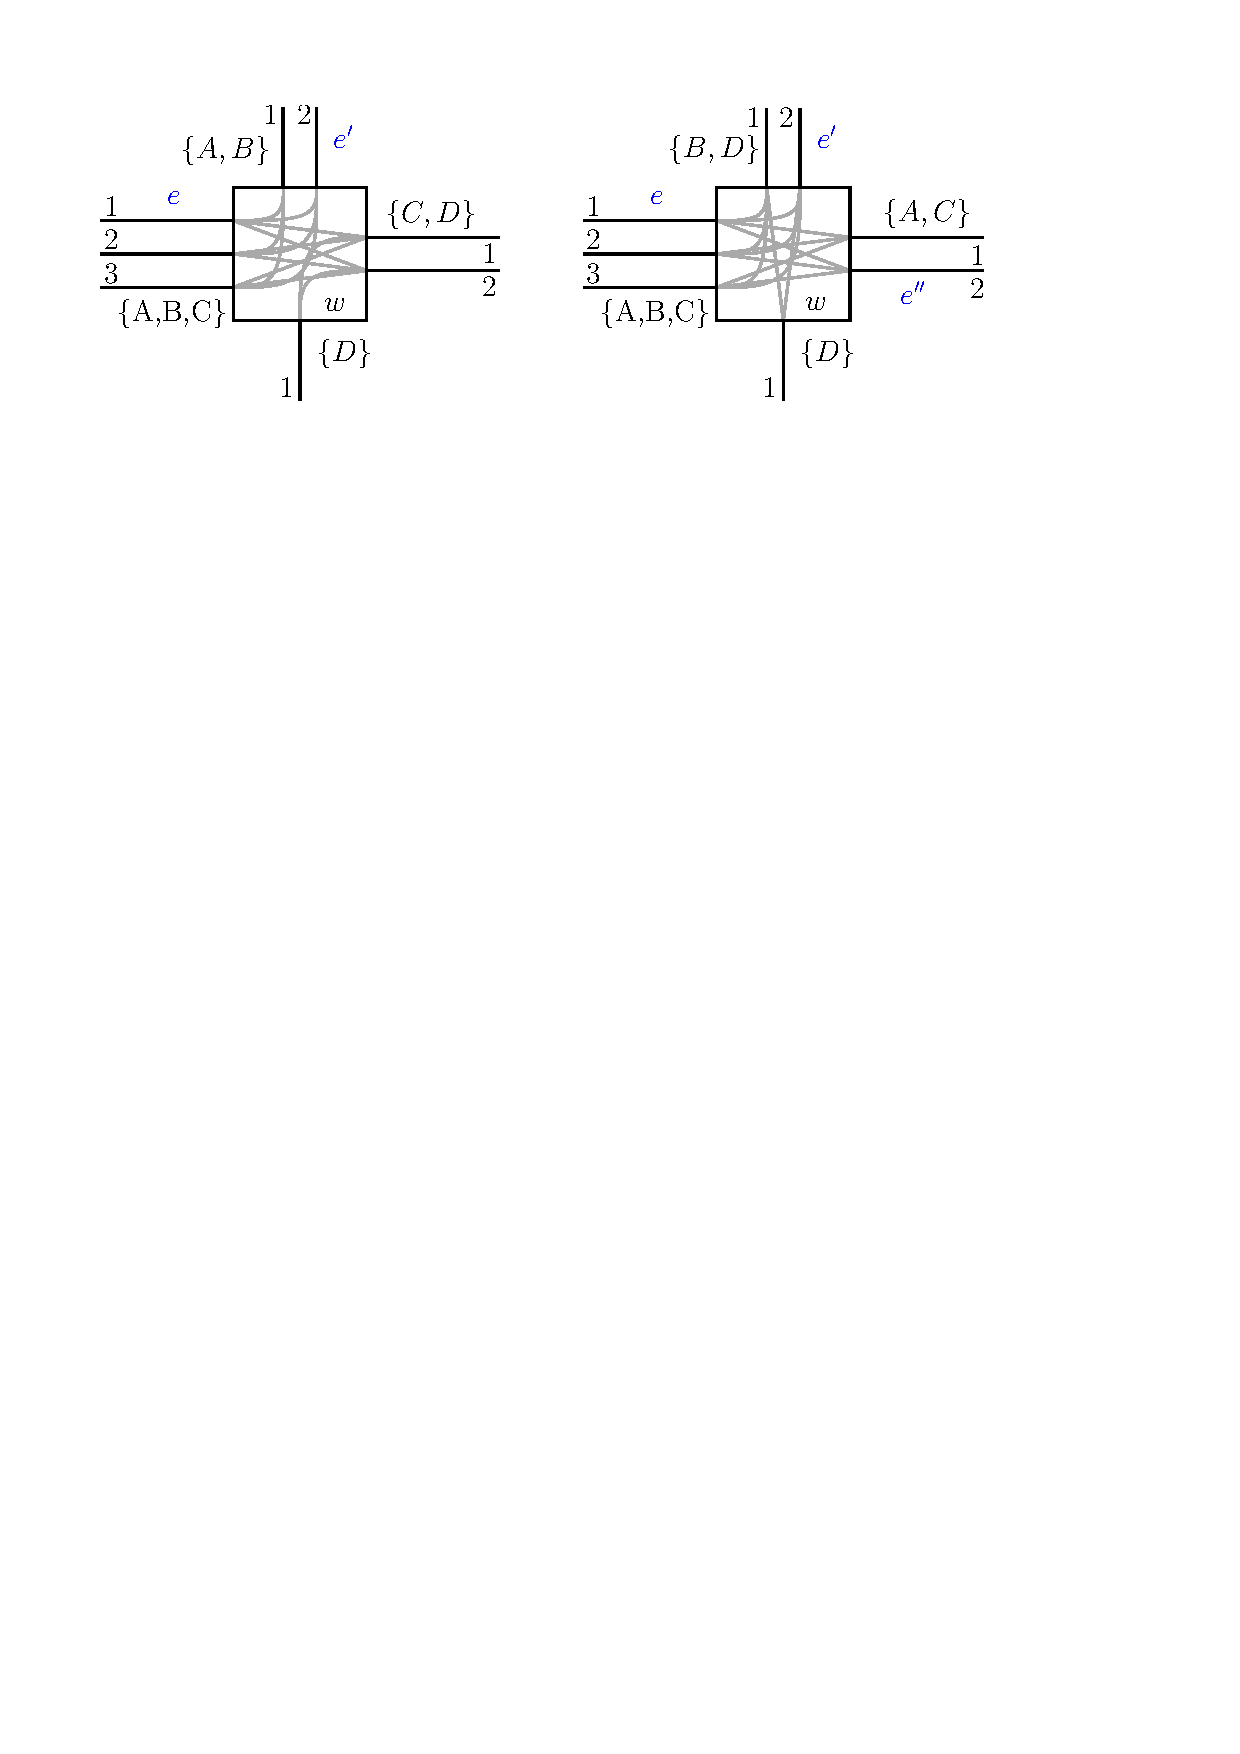
\includegraphics[width=0.66\textwidth]{crossing.pdf}}}$
	\caption{Line crossings of $\{A, B\}$ in the same segments (left) and into different segments (right) }
	\label{FIG:crossings}
\end{figure}
In the first case (left), $A, B$ induce a crossing if the position of $A$ is smaller than the position of $B$ in $s$ but vice versa in $s'$. We introduce the decision variable $x_{ss'AB} \in \{0,1\}$, which should be $1$ in case a crossing is induced and $0$ otherwise. To enforce this, we create one constraint per possible crossing as follows:
\begin{align*}
	x_{sA1} + x_{sB2} + x_{s'A2} + x_{s'B1} - x_{ss'AB} &\leq 3 \\
	x_{sA1} + x_{sB3} + x_{s'A2} + x_{s'B1} - x_{ss'AB} &\leq 3 \\
	x_{sA2} + x_{sB3} + x_{s'A2} + x_{s'B1} - x_{ss'AB} &\leq 3 \\
	x_{sA2} + x_{sB1} + x_{s'A1} + x_{s'B2} - x_{ss'AB} &\leq 3 \\
	x_{sA3} + x_{sB2} + x_{s'A1} + x_{s'B2} - x_{ss'AB} &\leq 3 \\
	x_{sA3} + x_{sB2} + x_{s'A1} + x_{s'B2} - x_{ss'AB} &\leq 3.
\end{align*}
In case one of the crossings occurs, the first four variables of the corresponding constraint all have to be 1. Hence their sum equals 4 and the only way to fulfill the $\leq 3$ constraint is to set $x_{ss'AB}$ to $1$.
The objective function then minimizes the sum over all such variables $x_{ss'AB}$.

In the second case (right), $A$ and $B$ split into different segments $s', s''$. Then the actual positions of $A$ and $B$ in $s', s''$ do not matter, but the order of $s'$ and $s''$ itself. So we introduce a split crossing decision variable $x_{ss's''AB} \in \{0,1\}$ and the following constraints:
\begin{align*}
	x_{sA1} + x_{sB2} - x_{ss's''AB} &\leq 1 \\
	x_{sA1} + x_{sB3} - x_{ss's''AB} &\leq 1 \\
	x_{sA2} + x_{sB3} - x_{ss's''AB} &\leq 1.
\end{align*}
Likewise, $x_{ss's''AB}$ is added to the objective function.

\subsubsection{ILP complexity}
Let $M = \max_{s \in S} |L(s)|$ be the maximum number of lines per segment. To get a mapping of lines to positions for each segment we need $\leq |S|M^{2}$ variables and $\leq 2|S|M$ constraints in total. To minimize crossings, we have to consider $\leq M^{2}$ pairs of lines per segment in $S$, and introduce a new decision variable for each such pair. That makes $\leq |S| M^{2}$ additional variables, which all appear in the objective function. Most constraints are introduced when both lines follow the same next segment. In that case, we create at most $\binom{M}{2}^{2} < M^{4}$ additional constraints per line pair per segment, so $\leq |S| M^{6}$ in total.

In summary, there are $\mathcal{O}(|S|M^{2})$ variables and $\mathcal{O}(|S|M^{6})$ constraints.

%
\subsection{Improved ILP}\label{SEC:improved}
%
The $\mathcal{O}(|S|M^{2})$ variables in the baseline ILP seem to be reasonable, as indeed $\Omega(|S|M^{2})$ crossings could occur. But the $\mathcal{O}(|S|M^{6})$ constraints are due to enumerating all possible position inversions explicitly. If on the other hand the statement \emph{position of A on $s$ is smaller than the position of B} would be efficiently checkable, the number of constraints could be reduced. To have such an oracle, we first modify the line-position assignment constraints. Subsequently, we use  the oracle to encode inversions with fewer constraints.

\subsubsection{Alternative line-position assignment}
Instead of a decision variable which encode the exact position of a line in a segment as before, we know use $x_{sl\leq p} \in \{0,1\}$ which is $1$ if the position of $l$ in $s$ is $\leq p$ and $0$ otherwise. To enforce a unique position, we use the constraints:
\begin{align}
	\forall l \in L(s) \forall p \in \{1, \cdots, |L(s)|-1\}: x_{sl\leq p} \leq x_{sl\leq p+1} \label{EQ:up_constr}
\end{align}
This ensures that the sequence can only switch from $0$ to $1$, and this exactly once. To make sure that at some point a $1$ appears and that each position is occupied by exactly one line, we additionally introduce the following constraints:
\begin{align}
	\forall p \in \{1, \cdots, |L(s)|\}: \sum_{l \in L(s)} x_{sl\leq p} = p \label{EQ:01_constr}
\end{align}
So exactly for  one line $x_{s.\leq 1} =1$ is true, for two lines $x_{s.\leq 2} = 1$ (of which one has to fulfill $x_{s.\leq 1} =1$) and so on.

\subsubsection{Crossing Oracle}
We reconsider the example from \ref{SEC:ac}, left. Before, we enumerated all possible positions which induce a crossing for $A, B$ at the transition from $s$ to $s'$. But it would be sufficient to have variables which tell us whether the position of $A$ is smaller than the position of $B$ in $s$, and the same for $s'$, and then compare those variables. For a line pair $(A,B)$ on segment $s$ we call the respective variables $x_{sA>B}, x_{sA<b} \in \{0, 1\}$. Since we introduce these variables for each line pair in $s$, $x_{sA<B}$ will re-appear as $x_{sB>A}$, so we only need $x_{sA>B}$. To get the desired value assignments, we add the following constraints:
\begin{gather}
	\sum_{p=1}^{|L(s)|} x_{sA\leq p} - \sum_{p} x_{sB\leq p} + x_{sA>B} M \geq 0 \\
	x_{sA>B} + x_{sB>A}=1.
\end{gather}
The equality constraints make sure that not both $x_{sA>B}$ and $x_{sB>A}$ can be $1$. If the position of $A$ is smaller than the position of $B$, then more of the variables corresponding to $A$ are $1$, hence the sum over all is higher. So if we subtract the sum for $B$ from the sum for $A$ and the result is $\geq 0$, we know the position of $A$ is  smaller and $x_{sA>B}$ can be $0$. Otherwise, the difference is negative, and we need to set $x_{sA>B}$ to $1$ to fulfill the inequality. It is then indeed fulfilled for sure as the position gap can never exceed the number of lines per segment.

To finally decide if there is a crossing, we would again like to have a decision variable $x_{ss'AB} \in \{0,1\}$ which is $1$ in case of a crossing and $0$ otherwise -- and minimize the sum of all such variables in the objective function.
The constraint
\begin{gather}
	abs(x_{sA<B}-x_{s'A<B}) - x_{ss'AB} \leq 0
\end{gather}
would realize this, as either $x_{sA<B} = x_{s'A<B}$ (both $0$ or both $1$) and then $x_{ss'AB}$ can be $0$, or they are unequal and hence the absolute value of their difference is $1$, enforcing $x_{ss'AB}=1$ to fulfill the $\leq 0$ condition. As absolute value computation can not be part of an ILP we use the following replacements:
\begin{align}
	x_{sA<B} - x_{s'A<B} - x_{ss'AB} &\leq 0 \label{EQ:abs_upper}\\
	-x_{sA<B} + x_{s'A<B} - x_{ss'AB} &\leq 0. \label{EQ:abs_lower}
\end{align}
If the values are equal, nothing changes in the argumentation. If the values are unequal, either (\ref{EQ:abs_upper}) or (\ref{EQ:abs_lower})  will produce a $1$ as the sum of the first two terms, enforcing $x_{ss'AB}=1$ as desired.

\subsubsection{Complexity of the improved ILP}
For the line-position assignment, we need at most $\leq |S|M^{2}$ variables and constraints just like in the basic formulation. For counting the  crossings, we need per pair of lines per segment only a constant number of new variables and constraints as shown above, hence $\mathcal{O}(|S|M^{2})$ in total.

\subsection{Placement of Inevitable Crossings}\label{SEC:crossing_placement}

Inevitable crossings are induced by the network's topology and have to occur somewhere. In the ILPs described above, the placement of these crossings largely depends on the solver's strategy.
However, we found that crossings should almost never happen inside of stations, as the crossing is then hidden behind a rendered station box and the semantic aspects of it are almost entirely lost to the reader. It may also be confusing if an inevitable crossing between two lines appeared in a part of the map where only these two lines travel next to each other.

We found that favoring nodes that aren't stations ($v_\sigma = 0$) and have a higher count of incident edges as a location for crossings yields maps that appear more well-arranged.
Since these criteria are invariant to the orderings imposed on $S$, we can control the placements by simply introducing a weighting factor $k_{ss'}$ which is added with each $x_{ss'll'}$ to the objective function.
The value of $k_{ss'}$ depends on the node where $s$ and $s'$ meet and is set like described above.

\subsection{Preventing Line Partner Separation}\label{SEC:separation}
So far, we only optimized for the number of line crossings. This may not lead to the solution that is most visually pleasing. Consider the example given in Figure~\ref{FIG:linesplitting}. The number of line crossings (1) is indeed minimized in the left example. However, the intuitive information that A and B continue together after x is lost. In the right example, this information is preserved, but the number of line crossings is now 2.
\begin{figure}
  \centering
	$\vcenter{\hbox{
\includegraphics[width=0.36\textwidth]{render_examples/splitting_example_nonopt.pdf}}}$
	\hspace{10mm}
    $\vcenter{\hbox{
\includegraphics[width=0.36\textwidth]{render_examples/splitting_example.pdf}}}$
	\caption{Left: optimized only for line crossings, Right: optimized also for line separations, with slightly higher penalty than crossings}
	\label{FIG:linesplitting}
\end{figure}
A related problem can be seen in Figure \todo{insert figure}. Both solutions have the same number of line crossings (2), but the right one clearly looks better, because the crossing is done in one pass. In both cases, we could adress the problem by punishing the separation of lines. For two adjacent segments $s$ and $s'$ and a line pair $(A, B$) that continues from $s$ to $s'$, if $A$ and $B$ were placed next to each other in $s$ (were partners in $s$) but not anymore in $s'$, we want to add some penalty to the objective function. For this, we introduce a variable $x_{sA\|B} \in \{0, 1\}$. Let $p_{sA}$ be the position of $A$ in $s$ and $p_{sB}$ the position of $B$ in $s$. We want $s_{sA\|B}$ to be $1$ if $\left|p_{sA} - p_{sB}\right| = 0$ (if they occur next to each other) and $1$ otherwise. To get the desired assignments, we add the following constraints per line pair in $s$:
\begin{align}
	\sum_{p=1}^{|L(s)|} x_{sA\leq p} - \sum_{p} x_{sB\leq p} - x_{sA\|B} M &\leq 1 \label{EQ:sep_cstr_1} \\
	\sum_{p=1}^{|L(s)|} x_{sB\leq p} - \sum_{p} x_{sA\leq p} - x_{sA\|B} M &\leq 1. \label{EQ:sep_cstr_2}
\end{align}
If $p_{sA} = p_{sB}$, then the difference of the sums in both constraints is 0. If $|p_{sA} - p_{sB}| = 1$, then the sum difference in both constraints is $\leq 1$. If $|p_{sA} - p_{sB}| > 1$, then either (\ref{EQ:sep_cstr_1}) or (\ref{EQ:sep_cstr_2}) enforce $x_{sA\|B} = 1$. To prevent the trivial solution where $x_{A\|B}$ is 1 for all line pairs, we introduce the following additional constraint per segment:
\begin{align}
	\sum_{l \in L(s)}\sum_{l' \in L(s)} x_{sl\|l'} \leq |L(s)|^2 - 3|L(s)| - 2
\end{align}
as indeed the maximal number of line pairs in $s$ (excluding lines paired with themselves) is $|L(s)|^2 - |L(s)$ and the number of $x_{sl\|l'}$ in $s$ that are 0 is exactly $2|L(s)| - 2$ (each line is next to its two neighbors, but the first and last line only have 1 neighbor). A fixed constraint is not necessary here, however, because the lower bound is already provided by the line pair constraints (\ref{EQ:sep_cstr_1}) and (\ref{EQ:sep_cstr_2}).

Like in Section~\ref{SEC:improved}, we introduce a decision variable $x_{ss'A\|B} \in \{0, 1\}$ that should be $1$ if $A$ and $B$ are splitted between $s$ and $s'$ and $0$ otherwise:
\begin{align}
	x_{sA\|B} - x_{s'A\|B} - x_{ss'A\|B} &\leq 0 \\
	-x_{sA\|B} + x_{s'A\|B} - x_{ss'A\|B} &\leq 0.
\end{align}
$x_{ss'A\|B}$ is added to the objective function. If $|L(s)| = |L(s')| = 2$, a line separation penalty is not needed for $A$ and $B$ because they will always be next to each other. If only $|L(s)| = 2$, we can add $x_{s'A\|B}$ to the objective function directly (and likewise if only $|L(s')|=2$).

\todo{Mention the special case of the MLCM-P periphery constraint the above constraints handle out-of-the-box}

\subsubsection{Complexity}
We add $1$ additional constraint per segment in $S$ and a constant number of additional constraints and variables per line pair to the ILP, so the number of variables and constraints is still in $\mathcal{O}(|S|M^2)$.

%
\subsection{Core problem graph}\label{SEC:coreprobgraph}
%
An inevitable crossing (or separation) between two lines $j$ and $k$ can only occur if there is at least one node with one of the following two properties:
\begin{enumerate}
\item $v$ is adjacent to segments $s : j \not\in L(s) \land k \in L(s')$ and $s' : j \in L(s') \land k \not\in L(s)$.
\item $|{s \in adj(v) : j \in L(s) \land i \in L(s)}| > 2$
\end{enumerate}
\textbf{Proof} (sketch): if no such $v_jk$ exists, then it holds for all nodes $v \in V$ that $j$ and $k$ either both travel through $v$ on the same two segments or they don't travel together through $v$ at all (or only one of them). In the latter case, no crossing (or separation) will occur and we can thus disregard it, which leaves us only with the former case. But if $j$ and $k$ travel through all nodes in which a crossing could occur together on the same two segments, then the relative order of $j$ and $k$ does not matter anymore - we just combine $j$ and $k$ into a new line $i$ and assign $j$ and $k$ an arbitrary (either $(j,k)$ or $(k, j$) global ordering.

We call nodes that comply to (1) for a line pair $A = \{j, k\}$ a liaison node for $j$ and $k$ and nodes that comply to (2) a T-node for $j$ and $k$. Additionally, we call a node that is a liaison and/or T-node for at least one line pair an \textbf{intersection node} and a node in which one or more lines end a \textbf{terminus node}.

Using the above, we can now greatly simplify the input graph prior to optimization with the following steps:
\begin{enumerate}
\item combine lines that always occur together and for which no intersection or T-node exists into a single line with a global, arbitrary relative ordering
\item delete each node with degree 2 (adjacent to segments $s = (u, v)$ and $s' = (v, w)$) and $L(s) = L(s')$ and combine $s$ and $s'$ into a single new segment $ss' = (u, w)$ with $L(ss') = L(s) = L(s')$ . Note that such a node can never be a terminus node or an intersection node.
\end{enumerate}
Since we never delete an intersection node, these operations will not affect the optimality of the found solution. In practice, they will "move" line crossings to nodes where a new line is introduced to an existing thread of lines (liaison nodes) or to nodes where topological changes are introduced to the network (T-nodes). This has a similar effect as the heuristic described in Section~\ref{SEC:crossing_placement}. For real-world networks, it can significantly reduce the number of ILP variables and constraints.

This core problem graph can be further prepared for optimiziation by splitting it into ordering-relevant connected components using the following rules:
\begin{enumerate}
	\item cut each segment $s = (u, v)$ with $|L(s)| = 1$ into two segments $s' = (u, v')$ and $s'' = (v'', v)$. Note that $v'$ and $v''$ are not connected.
	\item replace each segment $s = (u, v)$ where $v$ is a terminus node for each $l \in L(s)$ with a segment $s' = (u, v'$ where $v'$ is only connected to $s'$. Delete $s$ from the adjaceny list of $v$.
	\item remove each segment $s = (u, v)$ where $u$ and $v$ are termini for all $l \in L(s)$
\end{enumerate}
The line-ordering optimization can now be run independently on each connected component of the core problem graph, reducing the size of the ILPs that have to be solved and opening the way for parallelization.
\begin{figure}[h]
\centering
	\includestandalone[width=5cm]{tikz/transitgraph_optim}
	\hspace{0.6cm}
	\includestandalone[width=5cm]{tikz/coreoptimgraph}
	\caption{Left: transit graph $G$ with lines $a, b, c, d, e, f$, Right: core optimization graph with highlighted ordering-relevant connected components with more than 1 node; $ab$ was collapsed into $x$.}
\end{figure}

%
\section{Rendering}\label{SEC:rendering}
%
\todo{short explanation of parallel line rendering, node front expansion for non-station nodes, explain bezier curve and explain degeneration to circle arc}

%
\section{Evaluation}
%

%
\subsection{Optimization Results}
%

%
\subsection{Aesthetical Evaluation}
%

%
\section{Further work}
%
\bibliographystyle{plain}
\bibliography{tm.bib}

\end{document}
